\chapter{Architectural Design}

\section{Overview}

Travlendar+ has a multi-tier architecture.

\begin{figure}[H]
\begin{center}
\includegraphics[width=\textwidth, keepaspectratio]{"image/components".png}
\caption{High level components}
\end{center}
\end{figure}
 
User can interact directly with both version of the application: desktop and mobile, both laying on their respective OS APIs. The schedule computation is performed locally on the device in which the application runs by querying the GPS of the device and the external APIs:

\begin{itemize}
\item Mapping Service API
\item Travel Means APIs
\item Wheather Forecasts APIs
\end{itemize}

The communication between these components happens through different interfaces (wrappers), in order to improve the capability of the system to be expanded. In this way we provide a common pattern for the data acquired from the APIs, so that new ones can be easily included without the need of drastic changes on the central core.
In the architecture there are two more components: the Application server, that offers authentication and sinchronization services and the Database used to grant the durability of the data. At the end of the registration phase a new record is allocated in the Database and it will be used for check the identity of a user during the login phase. The Database also stores the user data (\ref{def:userdata}) so that they can be sinchronized in all the devices in which the user is logged in. 

\begin{figure}[H]
\begin{center}
\includegraphics[width=200pt, keepaspectratio]{"image/TierStack".png}
\caption{System stack}
\end{center}
\end{figure}

The figure above represents the stack architecture of our application and shows the hierarchy of the layers. Each level can communicate with the upper and lower layer.

\section{Component View}

\begin{figure}[H]
\begin{center}
\includegraphics[width=\textwidth, keepaspectratio, angle=90, origin=c]{"image/ComponentDiagram".png}
\caption{Component diagram}
\end{center}
\end{figure}


The application \footnote{in the image is reported only the mobile version of the application since the desktop version is identical to it, with the only difference that it can't exploit GPS services, so for mantaining the graphic clear only one of the two is reported.}
includes several components: 
\begin{itemize}

\item Identity Manager: it requests a service to the authentication provider either for the login or the registration of a user. 
%using the API offered by the OS it can communicate with the authentication manager that can write into the Database.

\item Appointment Manager: handles all the operations affecting appointment like modification, deletion and creation.
 
\item Scheduler: it computes and saves the schedules of the user.

\item Schedule Manager: handles all the operations affecting the schedule like showing and selecting the schedule to be run, notifying the user if a better schedule involving shared means has been found, buying the ticket for the means within the schedule. 

\item Runtime Schedule Manager: shows the directions and the progress of the running schedule.

\item Synchronization Manager: it requests a synchronization to the Synchronization provider when needed.

\item Mapping Service API Wrapper: manipulates data retrieved from a mapping service (e.g. Google Maps)in a format recognized by the application.

\item Travel Mean API Wrapper: manipulates data retrieved from a travel mean API service (e.g. Mobike, ATM, etc) in a format recognized by the application.

\item Weather Forecast API Wrapper: manipulates data retrieved from a weather forecast API service (e.g. Dark Sky) in a format recognized by the application.

\end{itemize}

The application Server is composed by the following two components:
\begin{itemize}

\item Authentication Provider: it handles the registration and the login phase of the user. 

\item Synchronization Provider: it has the purpose of synchronizing the user data (\ref{def:userdata}) in the database when something is changed.
 
\end{itemize}

The three components representing services (Wheather Forecast API, Travel Mean API, Mapping Service API) aren't included in the system because they are external services but they have been represented since our system is using the interfaces exposed from them.

\section{Deployment View}

\begin{figure}[H]
\begin{center}
\includegraphics[width=\textwidth, keepaspectratio]{"image/DeploymentDiagram".png}
\caption{Deployment Diagram}
\end{center}
\end{figure}

\section{Runtime View}

\begin{figure}[H]
\begin{center}
\includegraphics[width=\textwidth, keepaspectratio, angle=90,origin=c]{"image/RuntimeViews/Login".png}
\caption{Login runtime view}
\end{center}
\end{figure}

\begin{figure}[H]
\begin{center}
\includegraphics[width=\textwidth, keepaspectratio, angle=90,origin=c]{"image/RuntimeViews/AppointmentCreating".png}
\caption{Appointment creation runtime view}
\end{center}
\end{figure}

\begin{figure}[H]
\begin{center}
\includegraphics[width=\textwidth, keepaspectratio, angle=90,origin=c]{"image/RuntimeViews/AppointmentEditing".png}
\caption{Appointment editing runtime view}
\end{center}
\end{figure}

\begin{figure}[H]
\begin{center}
\includegraphics[width=\textwidth, keepaspectratio, angle=90,origin=c]{"image/RuntimeViews/DynamicDirections".png}
\caption{Dynamic directions runtime view}
\end{center}
\end{figure}

\begin{figure}[H]
\begin{center}
\includegraphics[width=\textwidth, keepaspectratio, angle=90,origin=c]{"image/RuntimeViews/Registration".png}
\caption{Registration runtime view}
\end{center}
\end{figure}

\begin{figure}[H]
\begin{center}
\includegraphics[width=710pt, keepaspectratio, angle=90,origin=c]{"image/RuntimeViews/ScheduleAppointments".png}
\caption{Schedule appointments runtime view}
\end{center}
\end{figure}

\begin{figure}[H]
\begin{center}

\includegraphics[width=\textwidth, keepaspectratio, angle=90,origin=c]{"image/RuntimeViews/RecoverCredentials".png}
\caption{Recover Credentials Runtime View}
\end{center}
\end{figure}

\begin{figure}[H]
\begin{center}
\includegraphics[width=\textwidth, keepaspectratio, angle=90,origin=c]{"image/RuntimeViews/BookingPhase".png}
\caption{Booking Phase Runtime View}
\end{center}
\end{figure}

\begin{figure}[H]
\begin{center}
\includegraphics[width=\textwidth, keepaspectratio, angle=90,origin=c]{"image/RuntimeViews/NotifySharedMeans".png}
\caption{Notify Shared Means Runtime View}
\end{center}
\end{figure}

%\begin{figure}[H]
%\begin{center}
%\includegraphics[width=720pt, keepaspectratio, angle=90,origin=c]{"image/RuntimeViews/ScheduleAppointments".png}
%\caption{Schedule Appointments Runtime View}
%\end{center}
%\end{figure} èDOPPIA

\begin{figure}[H]
\begin{center}
\includegraphics[width=720pt, keepaspectratio, angle=90,origin=c]{image/RuntimeViews/ScheduleSelection".png}
\caption{Schedule selection runtime view}
\end{center}
\end{figure}

\subsection{Note on Runtime Views}
In tbe diagrams the interaction involving Application Server, Application and API wrappers since they are not informative to show the behaviour of the application.

above only the interactions between internal components are shown.

\section{Component Interfaces}
\begin{figure}[H]
\begin{center}
\includegraphics[height=230pt, keepaspectratio, angle=90,origin=c]{image/InterfacesDiagrams".png}
\caption{Schedule selection runtime view}
\end{center}
\end{figure}

\section{ER Schema}
\begin{figure}[H]
\begin{center}
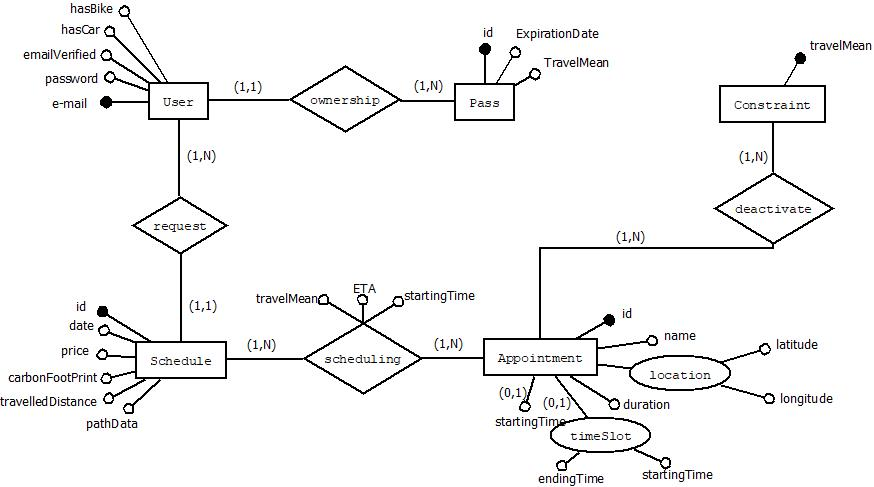
\includegraphics[width=580pt, keepaspectratio, angle=90,origin=c]{image/SchemaER/ER_DD.jpeg}
\caption{application database ER schema}
\end{center}
\end{figure}

\section{Selected architectural styles and patterns}

\begin{itemize}
\item MVC: all the classes of the application will adopt this pattern
\item Adapter: API wrappers will adopt this pattern
\item Client-Server: the application  running on a device represents the client part, reqesting services to the Travlendar server
\item OAuth: standard adopted by the exposed APIs of the server, in order to get authorization to make request from different clients
\item Restful API: a particular kind of APIs that encapsulate the request/response body in a JSON string
\item Singleton: restricts the instantiation of a class to one object. This is useful when exactly one object is needed to coordinate actions across the system. Some classes of our system can be built on this pattern, like the Travel Mean.
\end{itemize}


%\section{Other Design Decisions}
%
%\subsection{API Wrappers Class Diagrams}
%
%
%
%\begin{figure}[H]
%\begin{center}
%\includegraphics[width=\textwidth, keepaspectratio ,origin=c]{"image/WrapperUMLDiagram".png}
%\caption{API wrapper class diagram}
%\end{center}
%\end{figure}